\section{Funktionsweise}

\begin{frame}{Inversionsmethode}
	\begin{figure}
		\begin{subfigure}{.45\textwidth}
			\centering
			\includegraphics[width=\textwidth]{pdf_plots/logistic_-4to4.pdf}
            \caption{F mit Werten von $-4$ bis $4$}
		\end{subfigure}
		\begin{subfigure}{.45\textwidth}
			\centering
			\includegraphics[width=\textwidth]{pdf_plots/logistic_inv_0to1.pdf}
            \caption{F$^{-1}$ mit Werten von $0$ bis $1$}
		\end{subfigure}
	\end{figure}
\end{frame}

\begin{frame}{Inversionsmethode}
    \begin{itemize}
        \item Inverse einer Dichtefunktion benötigt 
        \item Entweder bekannt %\onslide<2->%, siehe \textit{\hyperref[tab:invFunctions]{Tabelle}} 
            oder numerisch integrierbar/annäherbar
    \end{itemize}
    \begin{table}%[htb!]
        \centering
        \begin{tabular}{l|l|l}
            Name         & Funktion & Zufällige Variable \\
            \hline\hline %& & \\
            Exponentiell & $1 - e^{-x}$ & $\log(1/U)$ \\ %\onslide<2->
            Logistisch   & $1 / (1 + e^{-x})$ & $-\log(\dfrac{1-U}{U})$ \\ %\onslide<3->
            Cauchy       & $1/2 + (1/\pi) \arctan(x)$ & $\tan(\pi U)$
        \end{tabular}
        \label{tab:invFunctions}
    \end{table}
\end{frame}

\begin{frame}{Hash-basierte Inversionsmethode}
    \dots
\end{frame}

\begin{frame}{Hash-basierte Inversionsmethode: Beispiel}
    \begin{figure}
        \centering
		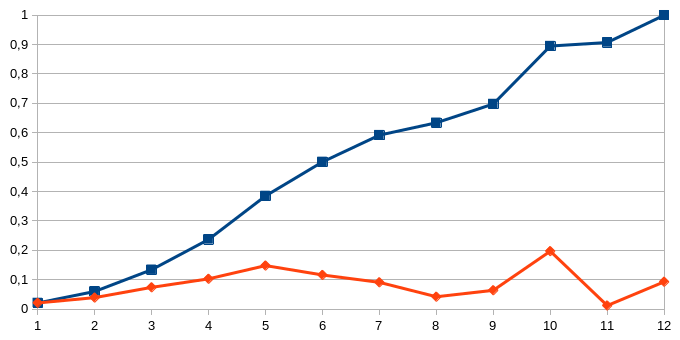
\includegraphics[width=.7\textwidth]{Screenshots/hashinv_exampleFuncPlot.png}
        \caption{Verteilungsfunktion F (orange) und ihre kummulative Dichte $\mathrm{C_F}$}
    \end{figure}
\end{frame}

\begin{frame}{Hash-basierte Inversionsmethode: Beispiel}
    \begin{table}%[htb!]
        \centering
        \begin{tabular}{l|l<{\onslide<2->}|l<{\onslide<3->}|c@{\hspace{\tabcolsep}\onslide<4->\onslide}}
            $X_j$   & $\mathrm{C_ F}(X_j)$  & $I_j$ & T$(I_j)$ \\
            \hline\hline % & & & \\
            $v_1$   & $0.021$   & $1$   & $1$ \\ 
            $v_2$   & $0.060$   & $1$   & $1$ \\
            $v_3$   & $0.134$   & $2$   & $3$ \\
            $v_4$   & $0.237$   & $3$   & $4$ \\
            $v_5$   & $0.385$   & $4$   & $5$ \\
            $v_6$   & $0.501$   & $6$   & $6$
        \end{tabular}
        \hspace{2em}
        \begin{tabular}{l|l<{\onslide<6->}|l<{\onslide<7->}|c@{\hspace{\tabcolsep}\onslide<8->\onslide<6->}}
            $X_j$   & $\mathrm{C_F}(X_j)$  & $I_j$ & T$(I_j)$ \\
            \hline\hline % & & & \\
            $v_7$   & $0.592$   & $6$   & $6$ \\ 
            $v_8$   & $0.634$   & $7$   & $8$ \\
            $v_9$   & $0.698$   & $7$   & $8$ \\
            $v_{10}$& $0.895$   & $9$   & $10$\\ 
            $v_{11}$& $0.907$   & $10$  & $11$\\
            $v_{12}$& $1.000$   & $11$  & $12$
        \end{tabular}
    \end{table}
\end{frame}

\begin{frame}{Hash-basierte Inversionsmethode: Beispiel}
    \begin{itemize}
        \item $u = 0.628$
        \begin{itemize}
            \item $I_u = \lfloor u * 10\rfloor + 1 = 7$
            \item $i = \mathrm{T}(I_u) = \mathrm{T}(7) = 8$
            \item $r$ ist nächstgrößerer Index, sodass T$(v_r)\neq \mathrm{T}(v_i)$, also $r = 10$
            \item F$v_{i-1} < u \leq \mathrm{F}(v_r)$
            \item $u < \mathrm{F}(v_8)\rightarrow X = v_8$
        \end{itemize}
    \end{itemize}
    
    
\end{frame}